\chapter{String algorithms}

This chapter deals with efficient algorithms
for string processing.
Many string problems can be easily solved
in $O(n^2)$ time, but the challenge is to
find algorithms that work in $O(n)$ or $O(n \log n)$
time.

\index{pattern matching}

For example, a fundamental problem related to strings
is the \key{pattern matching} problem:
given a string of length $n$ and a pattern of length $m$,
our task is to find the positions where the pattern
occurs in the string.
For example, the pattern \texttt{ABC} occurs two
times in the string \texttt{ABABCBABC}.

The pattern matching problem is easy to solve
in $O(nm)$ time by a brute force algorithm that
goes through all positions where the pattern may
occur in the string.
However, in this chapter, we will see that there
are more efficient algorithms that require only
$O(n+m)$ time.

\index{string}

\section{String terminology}

\index{alphabet}

An \key{alphabet} is a set of characters
that may appear in strings.
For example, the alphabet
$\{\texttt{A},\texttt{B},\ldots,\texttt{Z}\}$
consists of the capital letters of English.

\index{substring}

A \key{substring} is a sequence of consecutive
characters of a string.
The number of substrings of a string is $n(n+1)/2$.
For example, the substrings of the string
\texttt{ABCD} are
\texttt{A}, \texttt{B}, \texttt{C}, \texttt{D},
\texttt{AB}, \texttt{BC}, \texttt{CD},
\texttt{ABC}, \texttt{BCD} and \texttt{ABCD}.

\index{subsequence}

A \key{subsequence} is a sequence of
(not necessarily consecutive) characters
of a string in their original order.
The number of subsequences of a string is $2^n-1$.
For example, the subsequences of the string
\texttt{ABCD} are
\texttt{A}, \texttt{B}, \texttt{C}, \texttt{D},
\texttt{AB}, \texttt{AC}, \texttt{AD},
\texttt{BC}, \texttt{BD}, \texttt{CD},
\texttt{ABC}, \texttt{ABD}, \texttt{ACD},
\texttt{BCD} and \texttt{ABCD}.

\index{prefix}
\index{suffix}

A \key{prefix} is a subtring that starts at the beginning
of a string,
and a \key{suffix} is a substring that ends at the end
of a string.
For example, for the string \texttt{ABCD},
the prefixes are
\texttt{A}, \texttt{AB}, \texttt{ABC} and \texttt{ABCD}
and the suffixes are
\texttt{D}, \texttt{CD}, \texttt{BCD} and \texttt{ABCD}.

\index{rotation}

A \key{rotation} can be generated by moving
characters one by one from the beginning
to the end of a string (or vice versa).
For example, the rotations of the string
\texttt{ABCD} are
\texttt{ABCD}, \texttt{BCDA}, \texttt{CDAB} and \texttt{DABC}.

\index{period}

A \key{period} is a prefix of a string such that
the string can be constructed by repeating the period.
The last repetition may be partial and contain
only a prefix of the period.
For example, the shortest period of
\texttt{ABCABCA} is \texttt{ABC}.

\index{border}

A \key{border} is a string that is both
a prefix and a suffix of a string.
For example, the borders of the string \texttt{ABACABA}
are \texttt{A}, \texttt{ABA} and \texttt{ABACABA}.

\index{lexicographical order}

Strings are usually compared using the \key{lexicographical order}
that corresponds to the alphabetical order.
It means that $x<y$ if either $x \neq y$ and $x$ is a prefix of $y$,
or there is a position $k$ such that
$x[i]=y[i]$ when $i<k$ and $x[k]<y[k]$.

\section{Trie structures}

\index{trie}

A \key{trie} is a tree structure that
maintains a set of strings.
Each string in a trie corresponds to
a chain of characters starting at
the root node.
If two strings have a common prefix,
they also have a common chain in the tree.

For example, consider the following trie:

\begin{center}
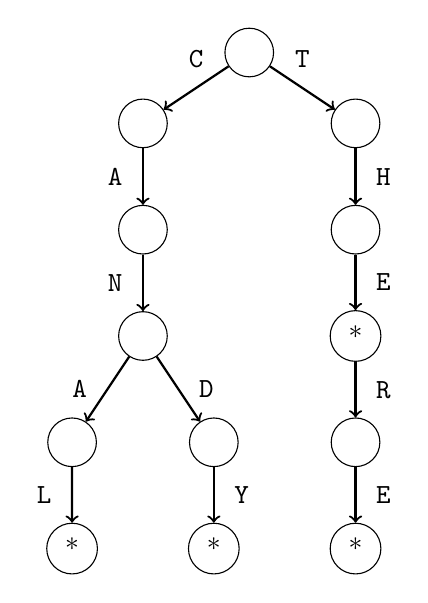
\begin{tikzpicture}[scale=0.9]
\node[draw, circle] (1) at (0,20) {$\phantom{1}$};
\node[draw, circle] (2) at (-1.5,19) {$\phantom{1}$};
\node[draw, circle] (3) at (1.5,19) {$\phantom{1}$};
\node[draw, circle] (4) at (-1.5,17.5) {$\phantom{1}$};
\node[draw, circle] (5) at (-1.5,16) {$\phantom{1}$};
\node[draw, circle] (6) at (-2.5,14.5) {$\phantom{1}$};
\node[draw, circle] (7) at (-0.5,14.5) {$\phantom{1}$};
\node[draw, circle] (8) at (-2.5,13) {*};
\node[draw, circle] (9) at (-0.5,13) {*};
\node[draw, circle] (10) at (1.5,17.5) {$\phantom{1}$};
\node[draw, circle] (11) at (1.5,16) {*};
\node[draw, circle] (12) at (1.5,14.5) {$\phantom{1}$};
\node[draw, circle] (13) at (1.5,13) {*};

\path[draw,thick,->] (1) -- node[font=\small,label=\texttt{C}] {} (2);
\path[draw,thick,->] (1) -- node[font=\small,label=\texttt{T}] {} (3);
\path[draw,thick,->] (2) -- node[font=\small,label=left:\texttt{A}] {} (4);
\path[draw,thick,->] (4) -- node[font=\small,label=left:\texttt{N}] {} (5);
\path[draw,thick,->] (5) -- node[font=\small,label=left:\texttt{A}] {} (6);
\path[draw,thick,->] (5) -- node[font=\small,label=right:\texttt{D}] {} (7);
\path[draw,thick,->] (6) -- node[font=\small,label=left:\texttt{L}] {}(8);
\path[draw,thick,->] (7) -- node[font=\small,label=right:\texttt{Y}] {} (9);
\path[draw,thick,->] (3) -- node[font=\small,label=right:\texttt{H}] {} (10);
\path[draw,thick,->] (10) -- node[font=\small,label=right:\texttt{E}] {} (11);
\path[draw,thick,->] (11) -- node[font=\small,label=right:\texttt{R}] {} (12);
\path[draw,thick,->] (12) -- node[font=\small,label=right:\texttt{E}] {} (13);
\end{tikzpicture}
\end{center}

This trie corresponds to the set
$\{\texttt{CANAL},\texttt{CANDY},\texttt{THE},\texttt{THERE}\}$.
The character * in a node means that
one of the strings in the set ends at the node.
This character is needed, because a string
may be a prefix of another string.
For example, in this trie, \texttt{THE}
is a prefix of \texttt{THERE}.

We can check if a trie contains a string
in $O(n)$ time where $n$ is the length of the string,
because we can follow the chain that starts at the root node.
We can also add a new string to the trie
in $O(n)$ time using a similar idea.
If needed, new nodes will be added to the trie.

Using a trie, we can also find
for a given string the longest prefix
that belongs to the set.
In addition, by storing additional information
in each node,
it is possible to calculate the number of
strings that have a given prefix.

A trie can be stored in an array
\begin{lstlisting}
int t[N][A];
\end{lstlisting}
where $N$ is the maximum number of nodes
(the maximum total length of the strings in the set)
and $A$ is the size of the alphabet.
The nodes of a trie are numbered
$1,2,3,\ldots$ so that the number of the root is 1,
and $\texttt{t}[s][c]$ is the next node in the chain
from node $s$ using character $c$.

\section{String hashing}

\index{hashing}
\index{string hashing}

\key{String hashing} is a technique that
allows us to efficiently check whether two
substrings in a string are equal\footnote{The technique
was popularized by the Karp–Rabin pattern matching
algorithm \cite{kar87}.}.
The idea is to compare the hash values of the
substrings instead of their individual characters.

\subsubsection*{Calculating hash values}

\index{hash value}
\index{polynomial hashing}

A \key{hash value} of a string is
a number that is calculated from the characters
of the string.
If two strings are the same,
their hash values are also the same,
which makes it possible to compare strings
based on their hash values.

A usual way to implement string hashing
is polynomial hashing, which means
that the hash value is calculated using the formula
\[(c[1] A^{n-1} + c[2] A^{n-2} + \cdots + c[n] A^0) \bmod B  ,\]
where $c[1],c[2],\ldots,c[n]$
are the codes of the characters in the string,
and $A$ and $B$ are pre-chosen constants.

For example, the codes of the characters
in the string \texttt{ALLEY} are:
\begin{center}
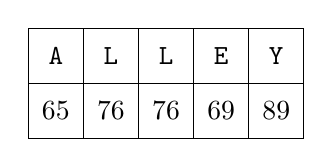
\begin{tikzpicture}[scale=0.7]
\draw (0,0) grid (5,2);

\node at (0.5, 1.5) {\texttt{A}};
\node at (1.5, 1.5) {\texttt{L}};
\node at (2.5, 1.5) {\texttt{L}};
\node at (3.5, 1.5) {\texttt{E}};
\node at (4.5, 1.5) {\texttt{Y}};

\node at (0.5, 0.5) {65};
\node at (1.5, 0.5) {76};
\node at (2.5, 0.5) {76};
\node at (3.5, 0.5) {69};
\node at (4.5, 0.5) {89};

\end{tikzpicture}
\end{center}

Thus, if $A=3$ and $B=97$, the hash value
for the string \texttt{ALLEY} is

\[(65 \cdot 3^4 + 76 \cdot 3^3 + 76 \cdot 3^2 + 69 \cdot 3^1 + 89 \cdot 3^0) \bmod 97 = 52.\]

\subsubsection*{Preprocessing}

To efficiently calculate hash values of substrings,
we need to preprocess the string.
It turns out that using polynomial hashing,
we can calculate the hash value of any substring
in $O(1)$ time after an $O(n)$ time preprocessing.

The idea is to construct an array $h$ such that
$h[k]$ contains the hash value of the prefix
of the string that ends at position $k$.
The array values can be recursively calculated as follows:
\[
\begin{array}{lcl}
h[0] & = & 0 \\
h[k] & = & (h[k-1] A + c[k]) \bmod B \\
\end{array}
\]
In addition, we construct an array $p$
where $p[k]=A^k \bmod B$:
\[
\begin{array}{lcl}
p[0] & = & 1 \\
p[k] & = & (p[k-1] A) \bmod B. \\
\end{array}
\]
Constructing these arrays takes $O(n)$ time.
After this, the hash value of a substring
that begins at position $a$ and ends at position $b$
can be calculated in $O(1)$ time using the formula
\[(h[b]-h[a-1] p[b-a+1]) \bmod B.\]

\subsubsection*{Using hash values}

We can efficiently compare strings using hash values.
Instead of comparing the individual characters of the strings,
the idea is to compare their hash values.
If the hash values are equal,
the strings are \emph{probably} equal,
and if the hash values are different,
the strings are \emph{certainly} different.

Using hashing, we can often make a brute force
algorithm efficient.
As an example, consider the pattern matching problem:
given a string $s$ and a pattern $p$,
find the positions where $p$ occurs in $s$.
A brute force algorithm goes through all positions
where $p$ may occur and compares the strings
character by character.
The time complexity of such an algorithm is $O(n^2)$.

We can make the brute force algorithm more efficient
using hashing, because the algorithm compares
substrings of strings.
Using hashing, each comparison only takes $O(1)$ time,
because only hash values of the strings are compared.
This results in an algorithm with time complexity $O(n)$,
which is the best possible time complexity for this problem.

By combining hashing and \emph{binary search},
it is also possible to find out the lexicographic order of
two strings in logarithmic time.
This can be done by calculating the length
of the common prefix of the strings using binary search.
Once we know the length of the common prefix,
we can just check the next character after the prefix,
because this determines the order of the strings.

\subsubsection*{Collisions and parameters}

\index{collision}

An evident risk when comparing hash values is
a \key{collision}, which means that two strings have
different contents but equal hash values.
In this case, an algorithm that relies on
the hash values concludes that the strings are equal,
but in reality they are not,
and the algorithm may give incorrect results.

Collisions are always possible,
because the number of different strings is larger
than the number of different hash values.
However, the probability of a collision is small
if the constants $A$ and $B$ are carefully chosen.
A usual way is to choose random constants
near $10^9$, for example as follows:
\[
\begin{array}{lcl}
A & = & 911382323 \\
B & = & 972663749 \\
\end{array}
\]

Using such constants,
the \texttt{long long} type can be used
when calculating the hash values,
because the products $AB$ and $BB$ will fit in \texttt{long long}.
But is it enough to have about $10^9$ different hash values?

Let us consider three scenarios where hashing can be used:

\textit{Scenario 1:} Strings $x$ and $y$ are compared with
each other.
The probability of a collision is $1/B$ assuming that
all hash values are equally probable.

\textit{Scenario 2:} A string $x$ is compared with strings
$y_1,y_2,\ldots,y_n$.
The probability of one or more collisions is

\[1-(1-\frac{1}{B})^n.\]

\textit{Scenario 3:} Strings $x_1,x_2,\ldots,x_n$
are compared with each other.
The probability of one or more collisions is
\[ 1 - \frac{B \cdot (B-1) \cdot (B-2) \cdots (B-n+1)}{B^n}.\]

The following table shows the collision probabilities
when $n=10^6$ and the value of $B$ varies:

\begin{center}
\begin{tabular}{rrrr}
constant $B$ & scenario 1 & scenario 2 & scenario 3 \\
\hline
$10^3$ & $0.001000$ & $1.000000$ & $1.000000$ \\
$10^6$ & $0.000001$ & $0.632121$ & $1.000000$ \\
$10^9$ & $0.000000$ & $0.001000$ & $1.000000$ \\
$10^{12}$ & $0.000000$ & $0.000000$ & $0.393469$ \\
$10^{15}$ & $0.000000$ & $0.000000$ & $0.000500$ \\
$10^{18}$ & $0.000000$ & $0.000000$ & $0.000001$ \\
\end{tabular}
\end{center}

The table shows that in scenario 1,
the probability of a collision is negligible
when $B \approx 10^9$.
In scenario 2, a collision is possible but the
probability is still quite small.
However, in scenario 3 the situation is very different:
a collision will almost always happen when
$B \approx 10^9$.

\index{birthday paradox}

The phenomenon in scenario 3 is known as the
\key{birthday paradox}: if there are $n$ people
in a room, the probability that some two people
have the same birthday is large even if $n$ is quite small.
In hashing, correspondingly, when all hash values are compared
with each other, the probability that some two
hash values are equal is large.

We can make the probability of a collision
smaller by calculating \emph{multiple} hash values
using different parameters.
It is unlikely that a collision would occur
in all hash values at the same time.
For example, two hash values with parameter
$B \approx 10^9$ correspond to one hash
value with parameter $B \approx 10^{18}$,
which makes the probability of a collision very small.

Some people use constants $B=2^{32}$ and $B=2^{64}$,
which is convenient, because operations with 32 and 64
bit integers are calculated modulo $2^{32}$ and $2^{64}$.
However, this is not a good choice, because it is possible
to construct inputs that always generate collisions when
constants of the form $2^x$ are used \cite{pac13}.

\section{Z-algorithm}

\index{Z-algorithm}
\index{Z-array}

The \key{Z-array} of a string
gives for each position $k$ in the string
the length of the longest substring
that begins at position $k$ and is a prefix of the string.
Such an array can be efficiently constructed
using the \key{Z-algorithm}\footnote{The Z-algorithm
was presented in \cite{gus97} as the simplest known
method for linear-time pattern matching, and the original idea
was attributed to \cite{mai84}.}.

For example, the Z-array for the string
\texttt{ACBACDACBACBACDA} is as follows:

\begin{center}
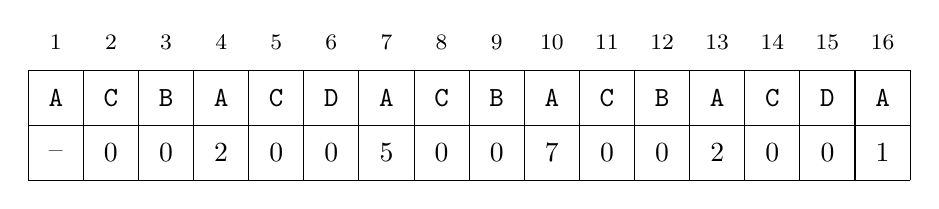
\begin{tikzpicture}[scale=0.7]
\draw (0,0) grid (16,2);

\node at (0.5, 1.5) {\texttt{A}};
\node at (1.5, 1.5) {\texttt{C}};
\node at (2.5, 1.5) {\texttt{B}};
\node at (3.5, 1.5) {\texttt{A}};
\node at (4.5, 1.5) {\texttt{C}};
\node at (5.5, 1.5) {\texttt{D}};
\node at (6.5, 1.5) {\texttt{A}};
\node at (7.5, 1.5) {\texttt{C}};
\node at (8.5, 1.5) {\texttt{B}};
\node at (9.5, 1.5) {\texttt{A}};
\node at (10.5, 1.5) {\texttt{C}};
\node at (11.5, 1.5) {\texttt{B}};
\node at (12.5, 1.5) {\texttt{A}};
\node at (13.5, 1.5) {\texttt{C}};
\node at (14.5, 1.5) {\texttt{D}};
\node at (15.5, 1.5) {\texttt{A}};

\node at (0.5, 0.5) {--};
\node at (1.5, 0.5) {0};
\node at (2.5, 0.5) {0};
\node at (3.5, 0.5) {2};
\node at (4.5, 0.5) {0};
\node at (5.5, 0.5) {0};
\node at (6.5, 0.5) {5};
\node at (7.5, 0.5) {0};
\node at (8.5, 0.5) {0};
\node at (9.5, 0.5) {7};
\node at (10.5, 0.5) {0};
\node at (11.5, 0.5) {0};
\node at (12.5, 0.5) {2};
\node at (13.5, 0.5) {0};
\node at (14.5, 0.5) {0};
\node at (15.5, 0.5) {1};

\footnotesize
\node at (0.5, 2.5) {1};
\node at (1.5, 2.5) {2};
\node at (2.5, 2.5) {3};
\node at (3.5, 2.5) {4};
\node at (4.5, 2.5) {5};
\node at (5.5, 2.5) {6};
\node at (6.5, 2.5) {7};
\node at (7.5, 2.5) {8};
\node at (8.5, 2.5) {9};
\node at (9.5, 2.5) {10};
\node at (10.5, 2.5) {11};
\node at (11.5, 2.5) {12};
\node at (12.5, 2.5) {13};
\node at (13.5, 2.5) {14};
\node at (14.5, 2.5) {15};
\node at (15.5, 2.5) {16};

\end{tikzpicture}
\end{center}

For example, the value at position 7 in the
above Z-array is 5,
because the substring \texttt{ACBAC} of length 5
is a prefix of the string,
but the substring \texttt{ACBACB} of length 6
is not a prefix of the string.

It is often a matter of taste whether to use
string hashing or the Z-algorithm.
Unlike hashing, the Z-algorithm always works
and there is no risk for collisions.
On the other hand, the Z-algorithm is more difficult
to implement and some problems can only be solved
using hashing.

\subsubsection*{Algorithm description}

The Z-algorithm scans the string from left
to right, and calculates for each position
the length of the longest substring that
is a prefix of the string.
A straightforward algorithm
would have a time complexity of $O(n^2)$,
but the Z-algorithm has an important
optimization which ensures that the time complexity
is only $O(n)$.

The idea is to maintain a range $[x,y]$ such that
the substring from $x$ to $y$ is a prefix of
the string and $y$ is as large as possible.
Since the Z-array already contains information
about the characters in the range $[x,y]$,
we can use this information to calculate
values for elements in the range $[x,y]$.

The time complexity of the Z-algorithm is $O(n)$,
because the algorithm only compares strings
character by character starting at position $y+1$.
If the characters match, the value of $y$ increases,
and it is not needed to compare the character at
position $y$ again
but the information in the Z-array can be used.

For example, let us construct the following Z-array:

\begin{center}
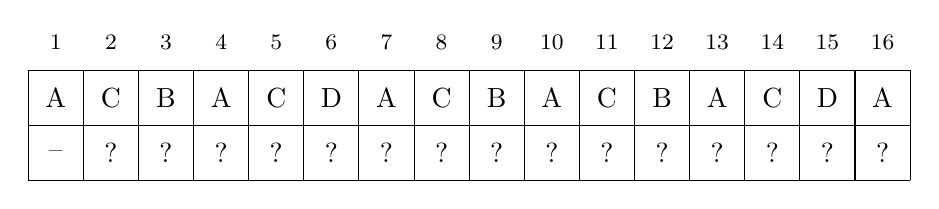
\begin{tikzpicture}[scale=0.7]
\draw (0,0) grid (16,2);

\node at (0.5, 1.5) {A};
\node at (1.5, 1.5) {C};
\node at (2.5, 1.5) {B};
\node at (3.5, 1.5) {A};
\node at (4.5, 1.5) {C};
\node at (5.5, 1.5) {D};
\node at (6.5, 1.5) {A};
\node at (7.5, 1.5) {C};
\node at (8.5, 1.5) {B};
\node at (9.5, 1.5) {A};
\node at (10.5, 1.5) {C};
\node at (11.5, 1.5) {B};
\node at (12.5, 1.5) {A};
\node at (13.5, 1.5) {C};
\node at (14.5, 1.5) {D};
\node at (15.5, 1.5) {A};

\node at (0.5, 0.5) {--};
\node at (1.5, 0.5) {?};
\node at (2.5, 0.5) {?};
\node at (3.5, 0.5) {?};
\node at (4.5, 0.5) {?};
\node at (5.5, 0.5) {?};
\node at (6.5, 0.5) {?};
\node at (7.5, 0.5) {?};
\node at (8.5, 0.5) {?};
\node at (9.5, 0.5) {?};
\node at (10.5, 0.5) {?};
\node at (11.5, 0.5) {?};
\node at (12.5, 0.5) {?};
\node at (13.5, 0.5) {?};
\node at (14.5, 0.5) {?};
\node at (15.5, 0.5) {?};

\footnotesize
\node at (0.5, 2.5) {1};
\node at (1.5, 2.5) {2};
\node at (2.5, 2.5) {3};
\node at (3.5, 2.5) {4};
\node at (4.5, 2.5) {5};
\node at (5.5, 2.5) {6};
\node at (6.5, 2.5) {7};
\node at (7.5, 2.5) {8};
\node at (8.5, 2.5) {9};
\node at (9.5, 2.5) {10};
\node at (10.5, 2.5) {11};
\node at (11.5, 2.5) {12};
\node at (12.5, 2.5) {13};
\node at (13.5, 2.5) {14};
\node at (14.5, 2.5) {15};
\node at (15.5, 2.5) {16};

\end{tikzpicture}
\end{center}

The first interesting position is 7 where the
length of the common prefix is 5.
After calculating this value,
the current $[x,y]$ range will be $[7,11]$:

\begin{center}
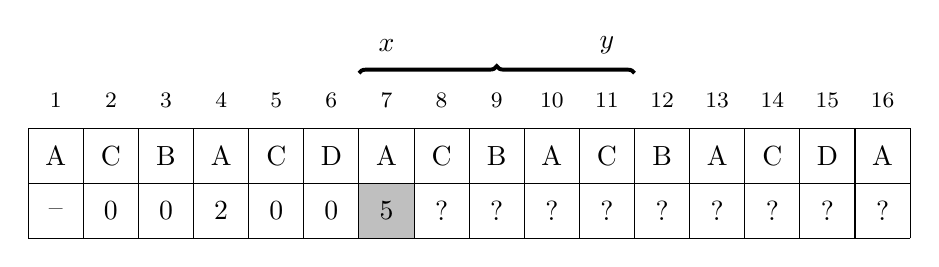
\begin{tikzpicture}[scale=0.7]
\fill[color=lightgray] (6,0) rectangle (7,1);
\draw (0,0) grid (16,2);

\node at (0.5, 1.5) {A};
\node at (1.5, 1.5) {C};
\node at (2.5, 1.5) {B};
\node at (3.5, 1.5) {A};
\node at (4.5, 1.5) {C};
\node at (5.5, 1.5) {D};
\node at (6.5, 1.5) {A};
\node at (7.5, 1.5) {C};
\node at (8.5, 1.5) {B};
\node at (9.5, 1.5) {A};
\node at (10.5, 1.5) {C};
\node at (11.5, 1.5) {B};
\node at (12.5, 1.5) {A};
\node at (13.5, 1.5) {C};
\node at (14.5, 1.5) {D};
\node at (15.5, 1.5) {A};

\node at (0.5, 0.5) {--};
\node at (1.5, 0.5) {0};
\node at (2.5, 0.5) {0};
\node at (3.5, 0.5) {2};
\node at (4.5, 0.5) {0};
\node at (5.5, 0.5) {0};
\node at (6.5, 0.5) {5};
\node at (7.5, 0.5) {?};
\node at (8.5, 0.5) {?};
\node at (9.5, 0.5) {?};
\node at (10.5, 0.5) {?};
\node at (11.5, 0.5) {?};
\node at (12.5, 0.5) {?};
\node at (13.5, 0.5) {?};
\node at (14.5, 0.5) {?};
\node at (15.5, 0.5) {?};

\draw [decoration={brace}, decorate, line width=0.5mm] (6,3.00) -- (11,3.00);

\node at (6.5,3.50) {$x$};
\node at (10.5,3.50) {$y$};


\footnotesize
\node at (0.5, 2.5) {1};
\node at (1.5, 2.5) {2};
\node at (2.5, 2.5) {3};
\node at (3.5, 2.5) {4};
\node at (4.5, 2.5) {5};
\node at (5.5, 2.5) {6};
\node at (6.5, 2.5) {7};
\node at (7.5, 2.5) {8};
\node at (8.5, 2.5) {9};
\node at (9.5, 2.5) {10};
\node at (10.5, 2.5) {11};
\node at (11.5, 2.5) {12};
\node at (12.5, 2.5) {13};
\node at (13.5, 2.5) {14};
\node at (14.5, 2.5) {15};
\node at (15.5, 2.5) {16};

\end{tikzpicture}
\end{center}

Now, it is possible to calculate the
subsequent values of the Z-array
more efficiently,
because we know that
the ranges $[1,5]$ and $[7,11]$
contain the same characters.
First, since the values at
positions 2 and 3 are 0,
we immediately know that
the values at positions 8 and 9
are also 0:

\begin{center}
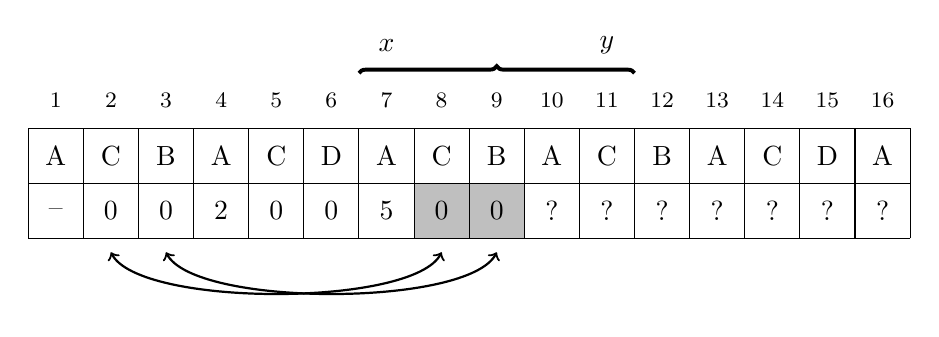
\begin{tikzpicture}[scale=0.7]
\fill[color=lightgray] (7,0) rectangle (9,1);
\draw (0,0) grid (16,2);

\node at (0.5, 1.5) {A};
\node at (1.5, 1.5) {C};
\node at (2.5, 1.5) {B};
\node at (3.5, 1.5) {A};
\node at (4.5, 1.5) {C};
\node at (5.5, 1.5) {D};
\node at (6.5, 1.5) {A};
\node at (7.5, 1.5) {C};
\node at (8.5, 1.5) {B};
\node at (9.5, 1.5) {A};
\node at (10.5, 1.5) {C};
\node at (11.5, 1.5) {B};
\node at (12.5, 1.5) {A};
\node at (13.5, 1.5) {C};
\node at (14.5, 1.5) {D};
\node at (15.5, 1.5) {A};

\node at (0.5, 0.5) {--};
\node at (1.5, 0.5) {0};
\node at (2.5, 0.5) {0};
\node at (3.5, 0.5) {2};
\node at (4.5, 0.5) {0};
\node at (5.5, 0.5) {0};
\node at (6.5, 0.5) {5};
\node at (7.5, 0.5) {0};
\node at (8.5, 0.5) {0};
\node at (9.5, 0.5) {?};
\node at (10.5, 0.5) {?};
\node at (11.5, 0.5) {?};
\node at (12.5, 0.5) {?};
\node at (13.5, 0.5) {?};
\node at (14.5, 0.5) {?};
\node at (15.5, 0.5) {?};


\draw [decoration={brace}, decorate, line width=0.5mm] (6,3.00) -- (11,3.00);

\node at (6.5,3.50) {$x$};
\node at (10.5,3.50) {$y$};


\footnotesize
\node at (0.5, 2.5) {1};
\node at (1.5, 2.5) {2};
\node at (2.5, 2.5) {3};
\node at (3.5, 2.5) {4};
\node at (4.5, 2.5) {5};
\node at (5.5, 2.5) {6};
\node at (6.5, 2.5) {7};
\node at (7.5, 2.5) {8};
\node at (8.5, 2.5) {9};
\node at (9.5, 2.5) {10};
\node at (10.5, 2.5) {11};
\node at (11.5, 2.5) {12};
\node at (12.5, 2.5) {13};
\node at (13.5, 2.5) {14};
\node at (14.5, 2.5) {15};
\node at (15.5, 2.5) {16};


\draw[thick,<->] (7.5,-0.25) .. controls (7,-1.25) and (2,-1.25) .. (1.5,-0.25);
\draw[thick,<->] (8.5,-0.25) .. controls (8,-1.25) and (3,-1.25) .. (2.5,-0.25);
\end{tikzpicture}
\end{center}

After this, we know that the value
at position 10 will be at least 2,
because the value at position 4 is 2:

\begin{center}
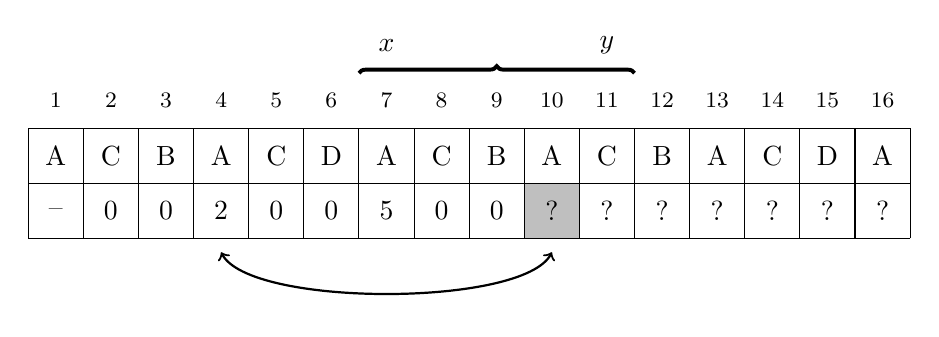
\begin{tikzpicture}[scale=0.7]
\fill[color=lightgray] (9,0) rectangle (10,1);
\draw (0,0) grid (16,2);

\node at (0.5, 1.5) {A};
\node at (1.5, 1.5) {C};
\node at (2.5, 1.5) {B};
\node at (3.5, 1.5) {A};
\node at (4.5, 1.5) {C};
\node at (5.5, 1.5) {D};
\node at (6.5, 1.5) {A};
\node at (7.5, 1.5) {C};
\node at (8.5, 1.5) {B};
\node at (9.5, 1.5) {A};
\node at (10.5, 1.5) {C};
\node at (11.5, 1.5) {B};
\node at (12.5, 1.5) {A};
\node at (13.5, 1.5) {C};
\node at (14.5, 1.5) {D};
\node at (15.5, 1.5) {A};

\node at (0.5, 0.5) {--};
\node at (1.5, 0.5) {0};
\node at (2.5, 0.5) {0};
\node at (3.5, 0.5) {2};
\node at (4.5, 0.5) {0};
\node at (5.5, 0.5) {0};
\node at (6.5, 0.5) {5};
\node at (7.5, 0.5) {0};
\node at (8.5, 0.5) {0};
\node at (9.5, 0.5) {?};
\node at (10.5, 0.5) {?};
\node at (11.5, 0.5) {?};
\node at (12.5, 0.5) {?};
\node at (13.5, 0.5) {?};
\node at (14.5, 0.5) {?};
\node at (15.5, 0.5) {?};

\draw [decoration={brace}, decorate, line width=0.5mm] (6,3.00) -- (11,3.00);

\node at (6.5,3.50) {$x$};
\node at (10.5,3.50) {$y$};


\footnotesize
\node at (0.5, 2.5) {1};
\node at (1.5, 2.5) {2};
\node at (2.5, 2.5) {3};
\node at (3.5, 2.5) {4};
\node at (4.5, 2.5) {5};
\node at (5.5, 2.5) {6};
\node at (6.5, 2.5) {7};
\node at (7.5, 2.5) {8};
\node at (8.5, 2.5) {9};
\node at (9.5, 2.5) {10};
\node at (10.5, 2.5) {11};
\node at (11.5, 2.5) {12};
\node at (12.5, 2.5) {13};
\node at (13.5, 2.5) {14};
\node at (14.5, 2.5) {15};
\node at (15.5, 2.5) {16};

\draw[thick,<->] (9.5,-0.25) .. controls (9,-1.25) and (4,-1.25) .. (3.5,-0.25);
\end{tikzpicture}
\end{center}

Since we have no information about the characters
after position 11, we have to begin to compare the strings
character by character:

\begin{center}
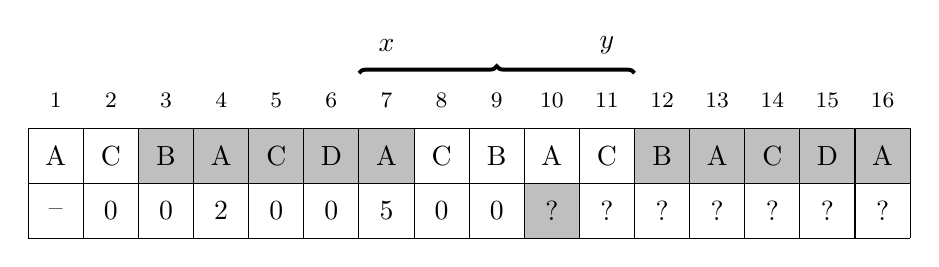
\begin{tikzpicture}[scale=0.7]
\fill[color=lightgray] (9,0) rectangle (10,1);
\fill[color=lightgray] (2,1) rectangle (7,2);
\fill[color=lightgray] (11,1) rectangle (16,2);


\draw (0,0) grid (16,2);

\node at (0.5, 1.5) {A};
\node at (1.5, 1.5) {C};
\node at (2.5, 1.5) {B};
\node at (3.5, 1.5) {A};
\node at (4.5, 1.5) {C};
\node at (5.5, 1.5) {D};
\node at (6.5, 1.5) {A};
\node at (7.5, 1.5) {C};
\node at (8.5, 1.5) {B};
\node at (9.5, 1.5) {A};
\node at (10.5, 1.5) {C};
\node at (11.5, 1.5) {B};
\node at (12.5, 1.5) {A};
\node at (13.5, 1.5) {C};
\node at (14.5, 1.5) {D};
\node at (15.5, 1.5) {A};

\node at (0.5, 0.5) {--};
\node at (1.5, 0.5) {0};
\node at (2.5, 0.5) {0};
\node at (3.5, 0.5) {2};
\node at (4.5, 0.5) {0};
\node at (5.5, 0.5) {0};
\node at (6.5, 0.5) {5};
\node at (7.5, 0.5) {0};
\node at (8.5, 0.5) {0};
\node at (9.5, 0.5) {?};
\node at (10.5, 0.5) {?};
\node at (11.5, 0.5) {?};
\node at (12.5, 0.5) {?};
\node at (13.5, 0.5) {?};
\node at (14.5, 0.5) {?};
\node at (15.5, 0.5) {?};

\draw [decoration={brace}, decorate, line width=0.5mm] (6,3.00) -- (11,3.00);

\node at (6.5,3.50) {$x$};
\node at (10.5,3.50) {$y$};


\footnotesize
\node at (0.5, 2.5) {1};
\node at (1.5, 2.5) {2};
\node at (2.5, 2.5) {3};
\node at (3.5, 2.5) {4};
\node at (4.5, 2.5) {5};
\node at (5.5, 2.5) {6};
\node at (6.5, 2.5) {7};
\node at (7.5, 2.5) {8};
\node at (8.5, 2.5) {9};
\node at (9.5, 2.5) {10};
\node at (10.5, 2.5) {11};
\node at (11.5, 2.5) {12};
\node at (12.5, 2.5) {13};
\node at (13.5, 2.5) {14};
\node at (14.5, 2.5) {15};
\node at (15.5, 2.5) {16};

%\draw[thick,<->] (11.5,-0.25) .. controls (11,-1.25) and (3,-1.25) .. (2.5,-0.25);
\end{tikzpicture}
\end{center}


It turns out that the length of the common
prefix at position 10 is 7,
and thus the new range $[x,y]$ is $[10,16]$:

\begin{center}
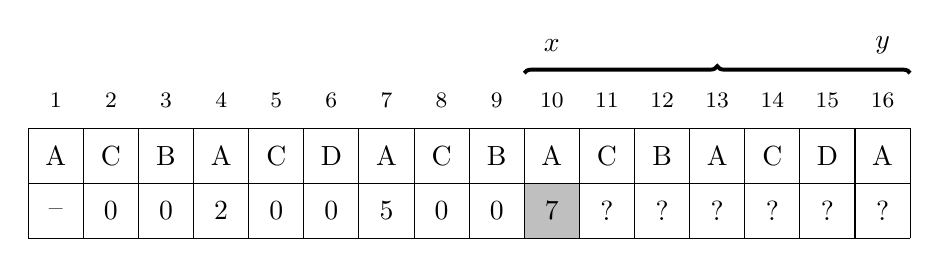
\begin{tikzpicture}[scale=0.7]
\fill[color=lightgray] (9,0) rectangle (10,1);
\draw (0,0) grid (16,2);

\node at (0.5, 1.5) {A};
\node at (1.5, 1.5) {C};
\node at (2.5, 1.5) {B};
\node at (3.5, 1.5) {A};
\node at (4.5, 1.5) {C};
\node at (5.5, 1.5) {D};
\node at (6.5, 1.5) {A};
\node at (7.5, 1.5) {C};
\node at (8.5, 1.5) {B};
\node at (9.5, 1.5) {A};
\node at (10.5, 1.5) {C};
\node at (11.5, 1.5) {B};
\node at (12.5, 1.5) {A};
\node at (13.5, 1.5) {C};
\node at (14.5, 1.5) {D};
\node at (15.5, 1.5) {A};

\node at (0.5, 0.5) {--};
\node at (1.5, 0.5) {0};
\node at (2.5, 0.5) {0};
\node at (3.5, 0.5) {2};
\node at (4.5, 0.5) {0};
\node at (5.5, 0.5) {0};
\node at (6.5, 0.5) {5};
\node at (7.5, 0.5) {0};
\node at (8.5, 0.5) {0};
\node at (9.5, 0.5) {7};
\node at (10.5, 0.5) {?};
\node at (11.5, 0.5) {?};
\node at (12.5, 0.5) {?};
\node at (13.5, 0.5) {?};
\node at (14.5, 0.5) {?};
\node at (15.5, 0.5) {?};

\draw [decoration={brace}, decorate, line width=0.5mm] (9,3.00) -- (16,3.00);

\node at (9.5,3.50) {$x$};
\node at (15.5,3.50) {$y$};


\footnotesize
\node at (0.5, 2.5) {1};
\node at (1.5, 2.5) {2};
\node at (2.5, 2.5) {3};
\node at (3.5, 2.5) {4};
\node at (4.5, 2.5) {5};
\node at (5.5, 2.5) {6};
\node at (6.5, 2.5) {7};
\node at (7.5, 2.5) {8};
\node at (8.5, 2.5) {9};
\node at (9.5, 2.5) {10};
\node at (10.5, 2.5) {11};
\node at (11.5, 2.5) {12};
\node at (12.5, 2.5) {13};
\node at (13.5, 2.5) {14};
\node at (14.5, 2.5) {15};
\node at (15.5, 2.5) {16};

% \draw[thick,<->] (9.5,-0.25) .. controls (9,-1.25) and (4,-1.25) .. (3.5,-0.25);
\end{tikzpicture}
\end{center}

After this, all subsequent values of the Z-array
can be calculated using the values already
stored in the array. All the remaining values can be
directly retrieved from the beginning of the Z-array:

\begin{center}
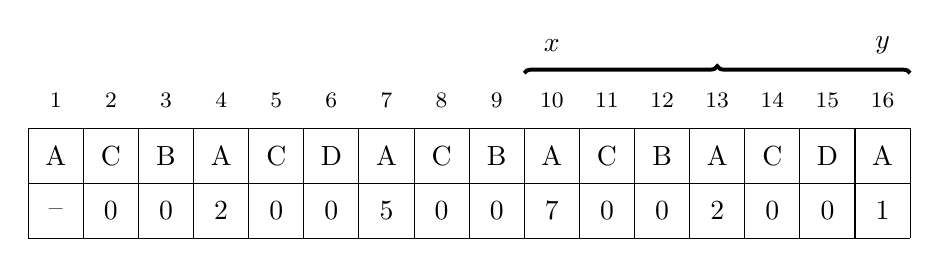
\begin{tikzpicture}[scale=0.7]
\draw (0,0) grid (16,2);

\node at (0.5, 1.5) {A};
\node at (1.5, 1.5) {C};
\node at (2.5, 1.5) {B};
\node at (3.5, 1.5) {A};
\node at (4.5, 1.5) {C};
\node at (5.5, 1.5) {D};
\node at (6.5, 1.5) {A};
\node at (7.5, 1.5) {C};
\node at (8.5, 1.5) {B};
\node at (9.5, 1.5) {A};
\node at (10.5, 1.5) {C};
\node at (11.5, 1.5) {B};
\node at (12.5, 1.5) {A};
\node at (13.5, 1.5) {C};
\node at (14.5, 1.5) {D};
\node at (15.5, 1.5) {A};

\node at (0.5, 0.5) {--};
\node at (1.5, 0.5) {0};
\node at (2.5, 0.5) {0};
\node at (3.5, 0.5) {2};
\node at (4.5, 0.5) {0};
\node at (5.5, 0.5) {0};
\node at (6.5, 0.5) {5};
\node at (7.5, 0.5) {0};
\node at (8.5, 0.5) {0};
\node at (9.5, 0.5) {7};
\node at (10.5, 0.5) {0};
\node at (11.5, 0.5) {0};
\node at (12.5, 0.5) {2};
\node at (13.5, 0.5) {0};
\node at (14.5, 0.5) {0};
\node at (15.5, 0.5) {1};

\draw [decoration={brace}, decorate, line width=0.5mm] (9,3.00) -- (16,3.00);

\node at (9.5,3.50) {$x$};
\node at (15.5,3.50) {$y$};


\footnotesize
\node at (0.5, 2.5) {1};
\node at (1.5, 2.5) {2};
\node at (2.5, 2.5) {3};
\node at (3.5, 2.5) {4};
\node at (4.5, 2.5) {5};
\node at (5.5, 2.5) {6};
\node at (6.5, 2.5) {7};
\node at (7.5, 2.5) {8};
\node at (8.5, 2.5) {9};
\node at (9.5, 2.5) {10};
\node at (10.5, 2.5) {11};
\node at (11.5, 2.5) {12};
\node at (12.5, 2.5) {13};
\node at (13.5, 2.5) {14};
\node at (14.5, 2.5) {15};
\node at (15.5, 2.5) {16};

\end{tikzpicture}
\end{center}

\subsubsection{Using the Z-array}

As an example, let us once again consider
the pattern matching problem,
where our task is to find the positions
where a pattern $p$ occurs in a string $s$.
We already solved this problem efficiently
using string hashing, but the Z-algorithm
provides another way to solve the problem.

A usual idea in string processing is to
construct a string that consists of
multiple strings separated by special characters.
In this problem, we can construct a string
$p$\texttt{\#}$s$,
where $p$ and $s$ are separated by a special
character \texttt{\#} that does not occur
in the strings.
The Z-array of $p$\texttt{\#}$s$ tells us the positions
where $p$ occurs in $s$,
because such positions contain the value $p$.

For example, if $s=$\texttt{HATTIVATTI} and $p=$\texttt{ATT},
the Z-array is as follows:

\begin{center}
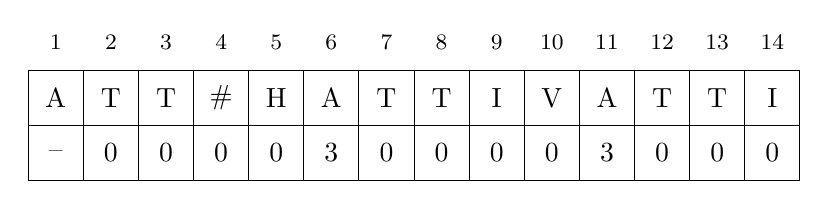
\begin{tikzpicture}[scale=0.7]
\draw (0,0) grid (14,2);

\node at (0.5, 1.5) {A};
\node at (1.5, 1.5) {T};
\node at (2.5, 1.5) {T};
\node at (3.5, 1.5) {\#};
\node at (4.5, 1.5) {H};
\node at (5.5, 1.5) {A};
\node at (6.5, 1.5) {T};
\node at (7.5, 1.5) {T};
\node at (8.5, 1.5) {I};
\node at (9.5, 1.5) {V};
\node at (10.5, 1.5) {A};
\node at (11.5, 1.5) {T};
\node at (12.5, 1.5) {T};
\node at (13.5, 1.5) {I};

\node at (0.5, 0.5) {--};
\node at (1.5, 0.5) {0};
\node at (2.5, 0.5) {0};
\node at (3.5, 0.5) {0};
\node at (4.5, 0.5) {0};
\node at (5.5, 0.5) {3};
\node at (6.5, 0.5) {0};
\node at (7.5, 0.5) {0};
\node at (8.5, 0.5) {0};
\node at (9.5, 0.5) {0};
\node at (10.5, 0.5) {3};
\node at (11.5, 0.5) {0};
\node at (12.5, 0.5) {0};
\node at (13.5, 0.5) {0};

\footnotesize
\node at (0.5, 2.5) {1};
\node at (1.5, 2.5) {2};
\node at (2.5, 2.5) {3};
\node at (3.5, 2.5) {4};
\node at (4.5, 2.5) {5};
\node at (5.5, 2.5) {6};
\node at (6.5, 2.5) {7};
\node at (7.5, 2.5) {8};
\node at (8.5, 2.5) {9};
\node at (9.5, 2.5) {10};
\node at (10.5, 2.5) {11};
\node at (11.5, 2.5) {12};
\node at (12.5, 2.5) {13};
\node at (13.5, 2.5) {14};
\end{tikzpicture}
\end{center}

The positions 6 and 11 contain the value 3,
which means that the pattern \texttt{ATT}
occurs in the corresponding positions
in the string \texttt{HATTIVATTI}.

The time complexity of the resulting algorithm
is $O(n)$, because it suffices to construct
the Z-array and go through its values.